\documentclass[11pt,oneside,leqno]{article}
\usepackage[paperwidth=6.5in,paperheight=9.5in,margin=.72in]{geometry}
\usepackage{fontspec}
\setmainfont{lmroman10-regular.otf}[BoldFont=lmroman10-bold.otf,ItalicFont=lmroman10-italic.otf,BoldItalicFont=lmroman10-bolditalic.otf,SmallCapsFont=lmromancaps10-regular.otf]
\usepackage{amsmath,amssymb,graphicx,tikz,microtype,needspace}
\usepackage[english]{babel}
\usepackage[unicode,hidelinks]{hyperref}
\hypersetup{pdftitle={Further Fragments on the Pentagramma mirificum},pdfauthor={Carl Friedrich Gauss}}
\newcommand{\SourceLeaf}[1]{\hypertarget{native-#1}{}}
\newcommand{\BareRoot}[1]{\mathord{\surd}#1}
\renewcommand{\thefootnote}{*)}
\setlength{\parindent}{1.2em}
\setlength{\emergencystretch}{1.4em}
\widowpenalty=10000\clubpenalty=10000\raggedbottom
\newcommand{\StepDown}[2]{\raisebox{-#1em}{$\displaystyle #2$}}
\newcommand{\TriLetter}[1]{\tikz[baseline=-.55ex,x=1ex,y=1ex,line width=.35pt]{\draw (0,0)--(2.1,2.1)--(4.2,0)--cycle;\node[inner sep=0pt] at (2.1,.65) {$\scriptstyle #1$};}}
\newcommand{\Arc}[1]{\overset{\frown}{#1}}
\newcommand{\HistAngle}{\mathord{\tikz[baseline=-.3ex,x=1ex,y=1ex,line width=.35pt]{\draw (1.35,1.0)--(0,.5)--(1.35,0);\draw (.18,1.18) .. controls (.85,.95) and (.85,.05) .. (.18,-.18);}}}
\begin{document}
\SourceLeaf{113}

\begin{center}\textbf{[FURTHER FRAGMENTS ON THE PENTAGRAMMA MIRIFICUM.]}\end{center}

\begin{center}\rule{1.5cm}{.4pt}\end{center}

\begin{center}[9.]\end{center}

The contraction exponents of the principal axes of the central projection ellipse are

\[
\sqrt{\dfrac{G'-1}{G'}} = \dfrac{2G'-1}{\sqrt{\alpha\beta\gamma\delta\varepsilon}} \quad \text{for the first axis } \dfrac{1}{\sqrt{G'}},
\]
\[
\sqrt{\dfrac{G''-1}{G''}} = \dfrac{2G''-1}{\sqrt{\alpha\beta\gamma\delta\varepsilon}} \quad \text{for the second axis } \dfrac{1}{\sqrt{G''}},
\]
or, since

\[
GG'G'' = -\tfrac14 \alpha\beta\gamma\delta\varepsilon,
\]
\[
(G-1)(G'-1)(G''-1) = -\tfrac14,
\]
\[
(2G-1)(2G'-1)(2G''-1) = -\alpha\beta\gamma\delta\varepsilon
\]
[hold], the contraction of the projected axes $= \dfrac{1}{1-2G}$.

It is advantageous to introduce, alongside the preceding quantities $G$, $G'$, $G''$, the roots of the following equation.

\[
\frac{u^3+u}{uu-1} = \sqrt{\alpha\beta\gamma\delta\varepsilon}
\]
If these are $\xi$, $\eta$, $\zeta$, then

\[
\xi+\eta+\zeta = -\xi\eta\zeta = \sqrt{\alpha\beta\gamma\delta\varepsilon},
\]
\[
\xi\eta+\eta\zeta+\zeta\xi = 1,
\]

\SourceLeaf{114}
\[
G = \frac{\zeta\zeta}{\zeta\zeta-1} \quad \text{or} \quad \zeta = \sqrt{\frac{G}{G-1}},
\]
\[
G' = \frac{\xi\xi}{\xi\xi-1} \quad \text{or} \quad \xi = \sqrt{\frac{G'}{G'-1}},
\]
\[
G'' = \frac{\eta\eta}{\eta\eta-1} \quad \text{or} \quad \eta = \sqrt{\frac{G''}{G''-1}}.
\]

\Needspace{8\baselineskip}The coordinates of the inner pentagon (the spherical one) are

\[
\frac{\dfrac{x}{\xi}}{\sqrt{\dfrac{xx}{\xi\xi}+\dfrac{yy}{\eta\eta}+\dfrac{zz}{\zeta\zeta}}}, \quad
\frac{\dfrac{y}{\eta}}{\sqrt{\dfrac{xx}{\xi\xi}+\dfrac{yy}{\eta\eta}+\dfrac{zz}{\zeta\zeta}}}, \quad
\frac{\dfrac{z}{\zeta}}{\sqrt{\dfrac{xx}{\xi\xi}+\dfrac{yy}{\eta\eta}+\dfrac{zz}{\zeta\zeta}}};
\]
those of the next inner pentagon would be

\[
\frac{\dfrac{x}{\xi\xi}}{\sqrt{\dfrac{xx}{\xi^4}+\dfrac{yy}{\eta^4}+\dfrac{zz}{\zeta^4}}}, \quad
\frac{\dfrac{y}{\eta\eta}}{\sqrt{\dfrac{xx}{\xi^4}+\dfrac{yy}{\eta^4}+\dfrac{zz}{\zeta^4}}}, \quad
\frac{\dfrac{z}{\zeta\zeta}}{\sqrt{\dfrac{xx}{\xi^4}+\dfrac{yy}{\eta^4}+\dfrac{zz}{\zeta^4}}}
\]
and so on. The coordinates of the outer pentagon, by contrast, are

\[
\frac{\xi x}{\sqrt{\xi\xi xx+\eta\eta yy+\zeta\zeta zz}}, \quad
\frac{\eta y}{\sqrt{\xi\xi xx+\eta\eta yy+\zeta\zeta zz}}, \quad
\frac{\zeta z}{\sqrt{\xi\xi xx+\eta\eta yy+\zeta\zeta zz}},
\]
and so on.

In our example, where $\alpha\beta\gamma\delta\varepsilon = 20$, the numerical values are

\[
\xi = 3{,}9276268 \qquad \eta = 1{,}3735071 \qquad \zeta = -0{,}8289980.
\]

\begin{center}\rule{3cm}{.4pt}\end{center}

\Needspace{12\baselineskip}\begin{center}[10.]\end{center}

$\lambda$, $\mu$ are contraction coefficients (negative fractions).

\[
\begin{aligned}
a,\; a\lambda,\; a\lambda\lambda,\; a\lambda^3,\; \ldots \\
b,\; b\mu,\; b\mu\mu,\; b\mu^3,\; \ldots
\end{aligned}
\Bigg\} \begin{gathered}\text{successive principal axes}\\\text{of the projection ellipses.}\end{gathered}
\]

$a\xi+b\eta i$, $a\xi'+b\eta' i$, etc., are the five points of the polygon (in star form).

$\lambda$, $\mu$, $\nu$ are roots of the equation

\[
\frac{\lambda\lambda+1}{\lambda^3-\lambda} = \frac{\mu\mu+1}{\mu^3-\mu} = \frac{\nu\nu+1}{\nu^3-\nu} = \sqrt{\alpha\beta\gamma\delta\varepsilon} = \frac{1}{\omega}.
\]

\SourceLeaf{115}

\[
\lambda+\mu+\nu=\lambda\mu\nu=\omega,
\]
\[
\lambda\mu+\mu\nu+\nu\lambda+1=0,
\]
\[
\lambda\lambda+\mu\mu+\nu\nu=\omega\omega+2.
\]
\[
\lambda=\operatorname{tang}\boldsymbol{L}, \qquad \mu=\operatorname{tang}\boldsymbol{M}, \qquad \nu=\operatorname{tang}\boldsymbol{N},
\]
\[
\boldsymbol{L}+\boldsymbol{M}+\boldsymbol{N}=0.
\]

In our example we have
\[
\boldsymbol{L}=-14^{0}17'4'', \qquad \boldsymbol{M}=-36^{0}3'26'', \qquad \boldsymbol{N}=50^{0}20'30''.
\]
\[
G'=\frac{1}{1-\lambda\lambda}=\frac{\cos \boldsymbol{L}^{2}}{\cos 2\boldsymbol{L}},
\]
\[
G''=\frac{1}{1-\mu\mu}=\frac{\cos \boldsymbol{M}^{2}}{\cos 2\boldsymbol{M}},
\]
\[
G\phantom{'}=\frac{1}{1-\nu\nu}=\frac{\cos \boldsymbol{N}^{2}}{\cos 2\boldsymbol{N}},
\]
\[
(1-\lambda\lambda)\xi\xi'+(1-\mu\mu)\eta\eta'+(1-\nu\nu)=0,
\]
\[
\left(\lambda+\frac{1}{\lambda}\right)\xi\xi'+\left(\mu+\frac{1}{\mu}\right)\eta\eta'+\left(\nu+\frac{1}{\nu}\right)=0,
\]
\[
\left(\lambda-\frac{1}{\lambda}\right)\xi\xi''+\left(\mu-\frac{1}{\mu}\right)\eta\eta''+\left(\nu-\frac{1}{\nu}\right)=0,
\]
\[
\frac{\lambda\lambda+1}{\lambda\lambda}\,\xi\xi''+\frac{\mu\mu+1}{\mu\mu}\,\eta\eta''+\frac{\nu\nu+1}{\nu\nu}=0,
\]
\[
\frac{\xi\xi'}{\sin 2\boldsymbol{L}}+\frac{\eta\eta'}{\sin 2\boldsymbol{M}}+\frac{1}{\sin 2\boldsymbol{N}}=0,
\]
\[
\frac{\xi\xi''}{\operatorname{tang} 2\boldsymbol{L}}+\frac{\eta\eta''}{\operatorname{tang} 2\boldsymbol{M}}+\frac{1}{\operatorname{tang} 2\boldsymbol{N}}=0.
\]

The four points $\lambda\xi+\mu\eta i$, $\xi'+\eta'i$, $\xi''+\eta''i$, $\lambda\xi'''+\mu\eta'''i$ lie on a straight line, and the same
holds for four other combinations of four other points each.

\[
\frac{\lambda\lambda+1}{\lambda}(\xi'''-\xi)\xi''''=\frac{\mu\mu+1}{\mu}(\eta-\eta''')\eta'''',
\]
\[
\frac{\lambda\lambda+1}{\lambda\lambda}(\xi'-\xi'')\xi''''=\frac{\mu\mu+1}{\mu\mu}(\eta''-\eta')\eta''''.
\]

\begin{center}\rule{3cm}{.4pt}\end{center}

\SourceLeaf{116}

\clearpage\begin{center}[11.]\end{center}

\noindent\begin{minipage}[t]{.46\textwidth}
\vspace{0pt}
\[
\begin{gathered}
\beta+\varepsilon+\lambda=\boldsymbol{A}, \\
\gamma+\alpha+\lambda=\boldsymbol{B}, \\
\delta+\beta+\lambda=\boldsymbol{C}, \\
\varepsilon+\gamma+\lambda=\boldsymbol{D}, \\
\alpha+\delta+\lambda=\boldsymbol{E},
\end{gathered}
\]

\[
\begin{gathered}
\gamma+\delta+\lambda=\boldsymbol{A}', \\
\delta+\varepsilon+\lambda=\boldsymbol{B}', \\
\varepsilon+\alpha+\lambda=\boldsymbol{C}', \\
\alpha+\beta+\lambda=\boldsymbol{D}', \\
\beta+\gamma+\lambda=\boldsymbol{E}',
\end{gathered}
\]

\end{minipage}\hfill\begin{minipage}[t]{.50\textwidth}
\vspace{0pt}
\begin{center}\resizebox{5.1cm}{!}{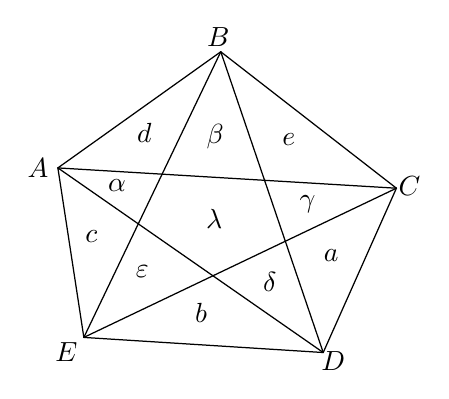
\begin{tikzpicture}[x=.006cm,y=-.006cm,line width=.45pt,line cap=round,line join=round,every node/.style={inner sep=0pt,font=\normalsize}]
\coordinate (A) at (177,347);
\coordinate (B) at (522,101);
\coordinate (C) at (894,390);
\coordinate (D) at (739,738);
\coordinate (E) at (232,706);
\draw (A) -- (B);
\draw (B) -- (C);
\draw (C) -- (D);
\draw (D) -- (E);
\draw (E) -- (A);
\draw (A) -- (C);
\draw (A) -- (D);
\draw (B) -- (E);
\draw (B) -- (D);
\draw (C) -- (E);
\node at (135,347) {$A$};
\node at (517,70) {$B$};
\node at (922,385) {$C$};
\node at (760,756) {$D$};
\node at (195,738) {$E$};
\node at (360,272) {$d$};
\node at (510,280) {$\beta$};
\node at (666,286) {$e$};
\node at (302,384) {$\alpha$};
\node at (706,424) {$\gamma$};
\node at (508,456) {$\lambda$};
\node at (248,493) {$c$};
\node at (356,566) {$\varepsilon$};
\node at (756,533) {$a$};
\node at (626,588) {$\delta$};
\node at (480,655) {$b$};
\end{tikzpicture}
}\end{center}

\[
\begin{gathered}
c+d+\alpha=\mathfrak{A}, \\
d+e+\beta=\mathfrak{B}, \\
e+a+\gamma=\mathfrak{C}, \\
a+b+\delta=\mathfrak{D}, \\
b+c+\varepsilon=\mathfrak{E},
\end{gathered}
\]
\end{minipage}


\[
a+b+c+d+e=s,
\]
\[
\alpha+\beta+\gamma+\delta+\varepsilon=\sigma,
\]
\[
\boldsymbol{A}+\boldsymbol{B}+\boldsymbol{C}+\boldsymbol{D}+\boldsymbol{E}=\boldsymbol{S}=\boldsymbol{A}'+\boldsymbol{B}'+\boldsymbol{C}'+\boldsymbol{D}'+\boldsymbol{E}',
\]
\[
\mathfrak{A}+\mathfrak{B}+\mathfrak{C}+\mathfrak{D}+\mathfrak{E}=\mathfrak{S},
\]
\[
\boldsymbol{S}=2\sigma+5\lambda=\boldsymbol{S}',
\]
\[
\mathfrak{S}=\sigma+2s, \qquad \omega=s+\sigma+\lambda.
\]

Proportionalities:
\[
a\boldsymbol{A}=(e+\gamma)(b+\delta),
\]
\[
b\boldsymbol{B}=(a+\delta)(c+\varepsilon),
\]
\[
c\boldsymbol{C}=(b+\varepsilon)(d+\alpha),
\]
\[
d\boldsymbol{D}=(c+\alpha)(e+\beta),
\]
\[
e\boldsymbol{E}=(d+\beta)(a+\gamma),
\]

\SourceLeaf{117}
all from the principle that the products of the opposite triangles (those
having only a common vertex or, more concisely, having no common side) into
which the diagonals divide a quadrilateral are equal.

The general barycentric equation among four points, e.\,g. $(A)$, $(B)$, $(C)$,
$(D)$, is
\[
\TriLetter{A}\,(A)+\TriLetter{B}\,(B)+\TriLetter{C}\,(C)+\TriLetter{D}\,(D)=0,
\]
where $\TriLetter{A}$ denotes the triangle $BCD$, $\TriLetter{B}$ the triangle $CDA$,
and so on (with due regard to [the] sign). In our case, if we add to the
preceding notation
\[
\boldsymbol{A}^{*}=\alpha+\gamma+\delta+a+\lambda, \quad \text{etc.}
\]
\[
\boldsymbol{A}^{*}=\omega-\mathfrak{B}-\mathfrak{E}, \quad \text{etc.},
\]
the equation among four points takes the form
\[
\mathfrak{C}(A)+\boldsymbol{D}^{*}(C)=\boldsymbol{A}^{*}(B)+\mathfrak{B}(D),
\]
where $(A)$ denotes the corresponding vertex of the outer pentagon. Equivalently, we have
\[
\begin{gathered}\mathfrak{C}(A)+(\omega-\mathfrak{E}-\mathfrak{C})(C)\\=(\omega-\mathfrak{B}-\mathfrak{E})(B)+\mathfrak{B}(D)\\=(\omega-\mathfrak{E})(e),\end{gathered}
\]
where $(e)$ denotes the corresponding point of the inner pentagon.

\begin{center}\rule{3cm}{.4pt}\end{center}

\begin{center}\resizebox{7cm}{!}{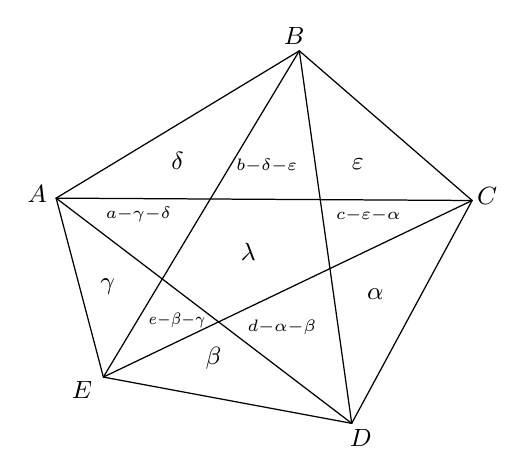
\begin{tikzpicture}[x=.006cm,y=-.006cm,line width=.45pt,line cap=round,line join=round,every node/.style={inner sep=0pt,font=\small}]
\coordinate (A) at (158,408);
\coordinate (B) at (673,96);
\coordinate (C) at (1039,413);
\coordinate (D) at (784,885);
\coordinate (E) at (258,787);
\draw (A) -- (B);
\draw (B) -- (C);
\draw (C) -- (D);
\draw (D) -- (E);
\draw (E) -- (A);
\draw (A) -- (C);
\draw (A) -- (D);
\draw (B) -- (E);
\draw (B) -- (D);
\draw (C) -- (E);
\node at (118,400) {$A$};
\node at (662,65) {$B$};
\node at (1071,403) {$C$};
\node at (803,916) {$D$};
\node at (213,814) {$E$};
\node at (415,330) {$\delta$};
\node at (604,339) {$\scriptstyle b-\delta-\varepsilon$};
\node at (797,337) {$\varepsilon$};
\node at (332,443) {$\scriptstyle a-\gamma-\delta$};
\node at (819,445) {$\scriptstyle c-\varepsilon-\alpha$};
\node at (565,522) {$\lambda$};
\node at (267,596) {$\gamma$};
\node at (414,666) {\scalebox{.86}[1]{$\scriptstyle e-\beta-\gamma$}};
\node at (491,747) {$\beta$};
\node at (636,681) {$\scriptstyle d-\alpha-\beta$};
\node at (834,612) {$\alpha$};
\end{tikzpicture}
}\end{center}

\[
\boldsymbol{A}c\varepsilon+\boldsymbol{C}c(b-\varepsilon)=\boldsymbol{B}b(c-\varepsilon)+\boldsymbol{D}b\varepsilon,
\]
\[
\boldsymbol{B}d\alpha+\boldsymbol{D}d(c-\alpha)=\boldsymbol{C}c(d-\alpha)+\boldsymbol{E}c\alpha,
\]
\[
\boldsymbol{C}e\beta+\boldsymbol{E}e(d-\beta)=\boldsymbol{D}d(e-\beta)+\boldsymbol{A}d\beta,
\]
\[
\boldsymbol{D}a\gamma+\boldsymbol{A}a(e-\gamma)=\boldsymbol{E}e(a-\gamma)+\boldsymbol{B}e\gamma,
\]
\[
\boldsymbol{E}b\delta+\boldsymbol{B}b(a-\delta)=\boldsymbol{A}a(b-\delta)+\boldsymbol{C}a\delta,
\]

\SourceLeaf{118}

\[
\lambda\alpha=(c-\alpha)(d-\alpha)-(e+b-\beta-\gamma-\delta-\varepsilon)\alpha,
\]
\[
\lambda \beta=(d-\beta)(e-\beta)-(a+c-\gamma-\delta-\varepsilon-\alpha)\beta,
\]
\[
\lambda \gamma=(e-\gamma)(a-\gamma)-(b+d-\delta-\varepsilon-\alpha-\beta)\gamma,
\]
\[
\lambda \delta=(a-\delta)(b-\delta)-(c+e-\varepsilon-\alpha-\beta-\gamma)\delta,
\]
\[
\lambda \varepsilon=(b-\varepsilon)(c-\varepsilon)-(d+a-\alpha-\beta-\gamma-\delta)\varepsilon,
\]
or in the following notation
\[
\lambda(0)=(8+9)(1+2)-0(3+7)
\]
or, if we set
\[
\alpha+\beta+\gamma+\delta+\varepsilon=\sigma, \qquad a+b+c+d+e=s
\]
then
\[
cd=(s+\lambda-\sigma-a)\alpha,
\]
\[
de=(s+\lambda-\sigma-b)\beta,
\]
\[
ea=(s+\lambda-\sigma-c)\gamma,
\]
\[
ab=(s+\lambda-\sigma-d)\delta,
\]
\[
bc=(s+\lambda-\sigma-e)\varepsilon.
\]

Thus [we obtain]
\[
\lambda=\omega-s+\frac{cd}{\omega-a}+\frac{de}{\omega-b}+\frac{ea}{\omega-c}+\frac{ab}{\omega-d}+\frac{bc}{\omega-e},
\]
\[
=\frac{acd}{\omega\omega-\omega a}+\frac{bde}{\omega\omega-\omega b}+\frac{cea}{\omega\omega-\omega c}+\frac{dab}{\omega\omega-\omega d}+\frac{ebc}{\omega\omega-\omega e}.
\]

Consequently, if we set $ab+bc+cd+de+ea=\boldsymbol{S}$ and $a\alpha+b\beta+c\gamma+d\delta+e\varepsilon=\Sigma$, then
\[
\boldsymbol{S}=\sigma(s+\lambda-\sigma)-\Sigma.
\]

The area of the outer polygon is $=s+\lambda-\sigma=\omega$. Hence
\[
\boldsymbol{S}=\sigma\omega-\Sigma.
\]

\begin{center}\rule{3cm}{.4pt}\end{center}

\clearpage\SourceLeaf{119}
\begin{center}\bfseries REMARKS ON THE ELEVEN\\PENTAGRAM FRAGMENTS.\end{center}

The numerous developments and notes on the »Pentagramma mirificum« found among
\textsc{Gauss}'s papers date from widely separated periods and vary considerably in their
notation. This variety corresponds to the many different points of view from which
\textsc{Gauss} considered the pentagram. In addition to the eight fragments published in
vol. III of the collected works, p. 481 ff., two further approaches are relevant here.
They form the basis of the three fragments printed above. Some further unpublished
developments contain in part
repetitions and in part detailed numerical calculations for the example that \textsc{Gauss}
repeatedly used, with $\alpha\beta\gamma\delta\varepsilon = 20$.

To explain the mathematical content of fragments [9] through [11], we need to go back
to fragments [1] through [8].

By »Pentagramma mirificum« \textsc{Gauss} means a spherical pentagon already used by \textsc{Neper}\footnote{Since
\textsc{Neper}'s investigations in question are relatively little known, we may be permitted
to say a few words about them here. They are found in Liber II,
Caput IV
of \textsc{Neper}'s »Mirifici Logarithmorum canonis descriptio« (Lugduni 1619) and
culminate in the theorem now known as »\textsc{Neper}'s rule«. If $h$ is the hypotenuse,
$a, b$ the legs of a right spherical triangle, and $\alpha, \beta$ the angles opposite
$a$ and $b$ respectively, then whenever $a, b, h, \alpha, \beta$ are such elements, the following
\[
a' = \frac{\pi}{2}-h, \qquad b' = \frac{\pi}{2}-\beta, \qquad h' = \frac{\pi}{2}-b, \qquad
\alpha' = \frac{\pi}{2}-a, \qquad \beta' = \alpha
\]
are also five elements of a right spherical triangle. The passage
from the first triangle to the second is an operation that closes on itself after five repetitions,
since we then return to the original elements
$a, b, h, \alpha, \beta$. \textsc{Neper} himself says that this rule follows plainly
from the figure of a pentagon of the very kind that \textsc{Gauss} studies in the fragments
under discussion. In fact, in the figure that will be described in more detail below, if we assign
to the triangle $P_1P_2Q_4$, taken on the sphere, the elements
$\Arc{P_1Q_4}=a$, $\Arc{P_2Q_4}=b$, $\Arc{P_1P_2}=h$, etc., then it is precisely the
adjacent right triangle $P_2P_3Q_5$ that acquires the elements just denoted by $a', b', h', \alpha',
\beta'$. We can thus take a single
right spherical triangle as our starting point and obtain from it, by
extending two sides by their complements and so on, the remaining four triangles of the
figure and hence the pentagram. ---} in his investigations of the right spherical triangle.
The pentagon has no reentrant angles. Each vertex is the pole of the opposite side,
and hence the five diagonals are quadrants of the sphere. All these
evidently self-polar pentagons form a doubly infinite continuum. The
accompanying figure shows, in stereographic projection, a pentagram
$P_1P_2P_3P_4P_5$.

\begin{center}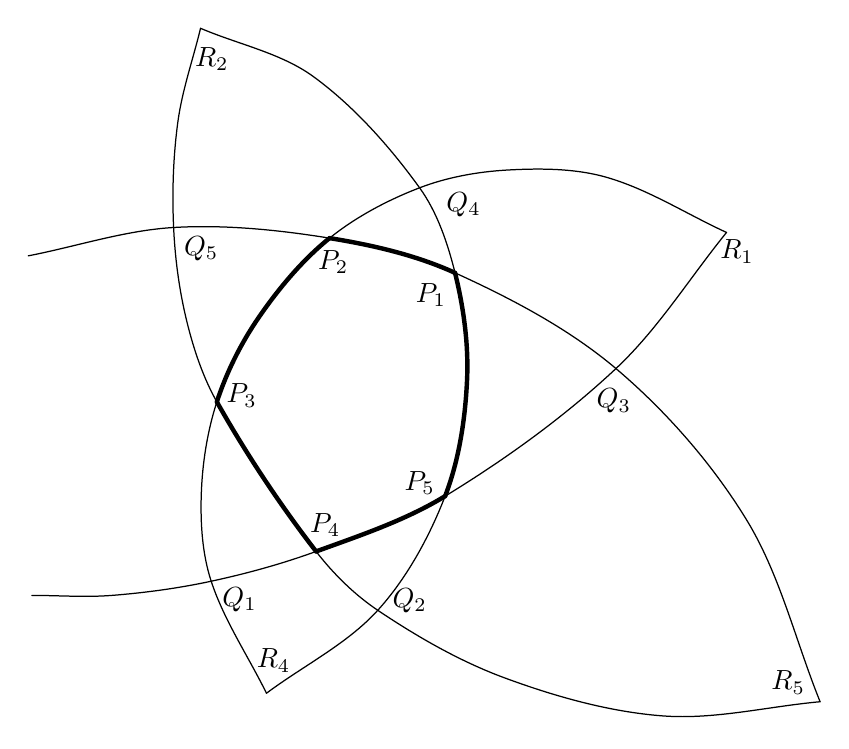
\begin{tikzpicture}[x=.009cm,y=-.009cm,line width=.45pt,line cap=round,line join=round,every node/.style={inner sep=0pt,font=\normalsize}]
\draw (30,336) .. controls (98.333,322.667) and (166.088,300.054) .. (235,296) .. controls (307.754,291.72) and (382.8,299.361) .. (455,311) .. controls (515.133,320.694) and (576.765,334.843) .. (632,360) .. controls (711.431,396.177) and (792.68,438.845) .. (859,495) .. controls (929.68,554.845) and (994.637,629.074) .. (1043,708) .. controls (1090.637,785.741) and (1112.333,879.333) .. (1147,965);
\draw[line width=1.6pt] (455,311) .. controls (515.133,320.694) and (576.765,334.843) .. (632,360);
\draw (35,815) .. controls (72.667,815) and (110.544,817.961) .. (148,815) .. controls (194.877,811.294) and (242.02,804.899) .. (288,795) .. controls (338.02,784.232) and (387.904,770.49) .. (436,753) .. controls (497.904,730.49) and (562.028,709.139) .. (618,675) .. controls (703.028,623.139) and (786.386,563.041) .. (859,495) .. controls (918.72,439.041) and (963,367) .. (1015,303);
\draw[line width=1.6pt] (436,753) .. controls (497.904,730.49) and (562.028,709.139) .. (618,675);
\draw (273,15) .. controls (262.333,59) and (247.038,102.352) .. (241,147) .. controls (234.371,196.019) and (232.728,246.548) .. (235,296) .. controls (237.062,340.882) and (243.206,386.471) .. (254,430) .. controls (263.54,468.471) and (276.537,507.458) .. (296,542) .. controls (337.203,615.124) and (384.695,686.552) .. (436,753) .. controls (460.362,784.552) and (490.015,813.844) .. (523,836) .. controls (578.348,873.177) and (638.442,907.813) .. (701,931) .. controls (772.442,957.48) and (849.434,979.239) .. (925,985) .. controls (998.101,990.573) and (1073,971.667) .. (1147,965);
\draw[line width=1.6pt] (296,542) .. controls (337.203,615.124) and (384.695,686.552) .. (436,753);
\draw (273,15) .. controls (326,37.667) and (386.337,49.75) .. (432,83) .. controls (489.337,124.75) and (540.299,182.245) .. (582,240) .. controls (606.966,274.578) and (621.666,318.357) .. (632,360) .. controls (644,408.357) and (651.209,460.287) .. (649,510) .. controls (646.543,565.287) and (637.872,623.584) .. (618,675) .. controls (595.872,732.251) and (564.027,790.74) .. (523,836) .. controls (480.027,883.406) and (418.333,914) .. (366,953);
\draw[line width=1.6pt] (632,360) .. controls (644,408.357) and (651.209,460.287) .. (649,510) .. controls (646.543,565.287) and (637.872,623.584) .. (618,675);
\draw (1015,303) .. controls (958.333,277) and (904.034,241.758) .. (845,225) .. controls (800.7,212.425) and (751.28,212.36) .. (705,215) .. controls (663.614,217.36) and (620.594,225.18) .. (582,240) .. controls (537.261,257.18) and (492.239,280.979) .. (455,311) .. controls (416.572,341.979) and (383.122,382.143) .. (355,423) .. controls (330.122,459.143) and (309.499,500.335) .. (296,542) .. controls (282.499,583.668) and (275.386,629.178) .. (274,673) .. controls (272.719,713.512) and (275.405,756.668) .. (288,795) .. controls (306.072,850.002) and (340,900.333) .. (366,953);
\draw[line width=1.6pt] (455,311) .. controls (416.572,341.979) and (383.122,382.143) .. (355,423) .. controls (330.122,459.143) and (309.499,500.335) .. (296,542);
\node at (289,58) {$R_2$};
\node at (1030,330) {$R_1$};
\node at (376,907) {$R_4$};
\node at (1102,938) {$R_5$};
\node at (274,326) {$Q_5$};
\node at (644,264) {$Q_4$};
\node at (856,541) {$Q_3$};
\node at (328,821) {$Q_1$};
\node at (568,823) {$Q_2$};
\node at (460,345) {$P_2$};
\node at (598,391) {$P_1$};
\node at (331,533) {$P_3$};
\node at (449,716) {$P_4$};
\node at (582,656) {$P_5$};
\end{tikzpicture}
\end{center}

It is accompanied by two further pentagons, winding twice and three times respectively,
$Q_1Q_3Q_5Q_2Q_4$ and $R_1R_4R_2R_5R_3$. By the fundamental property of the pentagram, the
angles of these two penta\SourceLeaf{120}gons are all right. If $s_k$ are the side lengths of the pentagram $P_1\ldots P_5$ (with
the radius of the sphere set equal to 1), the sides of the further pentagons are given by

\[
\Arc{P_kQ_{k+2}} = \frac{\pi}{2} - s_{k-2}, \qquad \Arc{P_kQ_{k-2}} = \frac{\pi}{2} - s_{k+2},
\]
\[
\Arc{Q_kR_{k+2}} = s_{k+1}, \qquad \Arc{Q_kR_{k-2}} = s_{k-1}.
\]

Among the pentagrams there is in particular a regular one. It has side length
$s = \operatorname{arc\,sin}\sqrt{\dfrac{-1+\sqrt{5}}{2}}$ and can be generated from the spherical triangle with
angles $\dfrac{2\pi}{5}, \dfrac{\pi}{2}, \dfrac{\pi}{4}$ by replication around the vertex of the
first angle.

The geometric relations just exhibited for the general pentagram can be written as a series of
equations by means of the fundamental formulas of the right spherical triangle.
This is done in fragments [1] and [3]. ---

If the pentagram is projected from the center of the sphere onto a tangent plane whose point of
tangency $O$ lies in the pentagram, the result is a plane pentagon in which the five
lines $\overline{OP_k}$ give the altitudes. The plane pentagon therefore has two properties,
which also determine it.

1) The five altitudes all pass through the same point $O$.

2) Each altitude is divided by $O$ into two segments whose product is the same for all altitudes,
namely the square of the radius of the sphere.

\textsc{Gauss} now takes the projection plane to represent the complex numbers (cf. fragment [2])
and chooses $O$ in particular as the origin. The subsequent developments in fragment [2]
have the following meaning. On five rays issuing from $O$, five
points $p, p', \ldots, p''''$ are chosen arbitrarily. The displacement described by \textsc{Gauss}
moves these points along their respective rays to the positions $q, q', \ldots, q''''$,
which are then the vertices of a pentagram of our kind. ---

If $M$ is the center of the sphere, the five rays to the vertices $P_k$ of the pentagram,
namely $\overline{MP_k}$, lie on a uniquely determined quadratic cone.
This cone, and especially its trans\SourceLeaf{121}formation to principal axes, play a fundamental role in \textsc{Gauss}'s subsequent
developments. The cubic equation for this principal-axis transformation, which
depends only on the product of the tangents of the pentagram's five sides, is also treated
numerically in [5]. To prove the numerous relations in
fragments [5] and [6], it is best to start from the familiar modern
fundamental formulas for the principal-axis transformation of a cone. In the coordinate system
originally chosen by \textsc{Gauss}, $x, y, z$, the equations of these fragments can be derived from those formulas
with almost no calculation. ---

The developments in [7] and [8], dated 1843 April 20, establish the
relation of the pentagram to the division of elliptic functions into fifths.
There can be no doubt that \textsc{Gauss} recognized this relation under the stimulus of \textsc{Jacobi}'s paper Ȇber die
Anwendung der elliptischen Transcendenten auf ein bekanntes Problem der
Elementargeometrie«\footnote{\textsc{Crelle}'s Journal, vol. 3 (1828).} \textsc{Jacobi} there studies
pentagons each inscribed in one circle and at the same time circumscribed about a second
circle, and shows their relation to elliptic functions.

To pass from the pentagram to \textsc{Jacobi}'s pentagon, project the
former from the center of the sphere onto the tangent plane to the sphere whose
point of tangency is the intersection of the sphere with the axis of the cone. The cone
meets this projection plane in an ellipse, in which the projected pentagram
is inscribed. The affine transformation shown in the accompanying figure gives,
in $P_1'P_2'\,..\,P_5'$, a \textsc{Jacobi} pentagon.

\begin{center}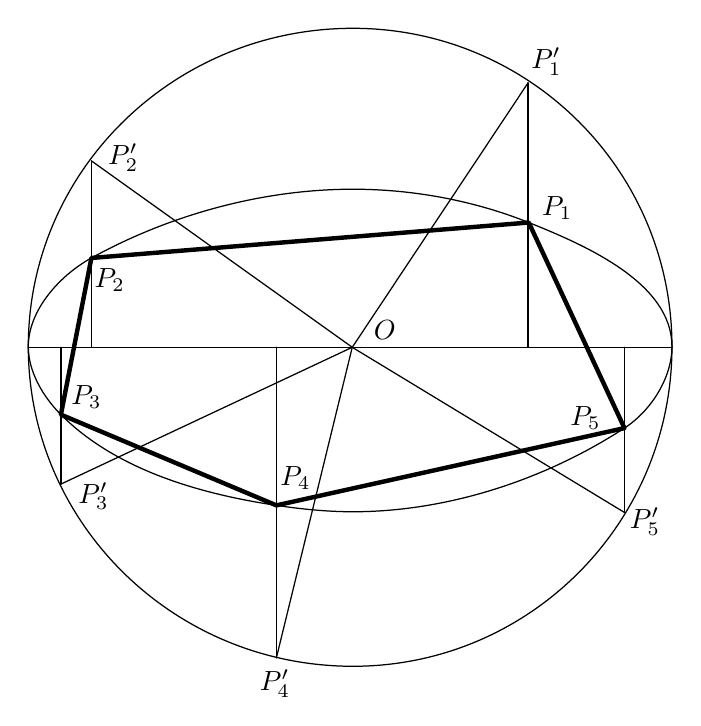
\begin{tikzpicture}[x=.009cm,y=-.009cm,line width=.45pt,line cap=round,line join=round,every node/.style={inner sep=0pt,font=\normalsize}]
\draw (41,480) .. controls (41,232) and (246,31) .. (499,31) .. controls (748,31) and (949,232) .. (949,480) .. controls (949,729) and (748,931) .. (499,931) .. controls (246,931) and (41,729) .. cycle;
\draw (41,480) .. controls (41,428.851) and (85.182,379.65) .. (130,355) .. controls (241.436,293.71) and (371.821,258) .. (499,258) .. controls (583.138,258) and (668.88,273.752) .. (747,305) .. controls (829.716,338.086) and (949,390.913) .. (949,480) .. controls (949,524.365) and (919.197,570.822) .. (882,595) .. controls (769.994,667.804) and (632.589,713) .. (499,713) .. controls (462.875,713) and (426.725,709.359) .. (391,704) .. controls (282.267,687.69) and (164.746,653.746) .. (87,576) .. controls (61.909,550.909) and (41,515.484) .. (41,480);
\draw (41,481)--(949,481);
\draw (498,481)--(746,108);
\draw (746,108)--(746,481);
\draw (498,481)--(130,218);
\draw (130,218)--(130,481);
\draw (498,481)--(87,674);
\draw (87,674)--(87,481);
\draw (498,481)--(391,919);
\draw (391,919)--(391,481);
\draw (498,481)--(882,714);
\draw (882,714)--(882,481);
\draw[line width=1.6pt] (747,305)--(130,355)--(87,576)--(391,704)--(882,595)--cycle;
\node at (772,78) {$P_1'$};
\node at (175,213) {$P_2'$};
\node at (133,691) {$P_3'$};
\node at (389,956) {$P_4'$};
\node at (911,727) {$P_5'$};
\node at (787,284) {$P_1$};
\node at (156,386) {$P_2$};
\node at (123,551) {$P_3$};
\node at (418,665) {$P_4$};
\node at (827,581) {$P_5$};
\node at (544,457) {$O$};
\end{tikzpicture}
\end{center}

These statements are confirmed by the agreement of \textsc{Gauss}'s formulas in [7]
and [8] with the equations derived by \textsc{Jacobi} in the cited work. To prove
\textsc{Gauss}'s relations, we can proceed as follows.

Use the principal axes of the ellipse as axes $x, y$ in the projection plane and set the
radius of the sphere equal to 1. The center of the sphere then lies directly below $O$ at a distance of
1 measured perpendicular to the plane. The fundamental property of the pentagram, namely
that $\HistAngle P_{k-1}MP_{k+1} = \dfrac{\pi}{2}$, gives the five equations

\[
x_{k-1}x_{k+1} + y_{k-1}y_{k+1} + 1 = 0,\tag{1}
\]
\SourceLeaf{122}where $x_k, y_k$ are the coordinates of $P_k$. Each pair $x_k, y_k$ appears in two
equations, which can be solved to give

\[
x_k = \dfrac{y_{k+2}-y_{k-2}}{x_{k+2}y_{k-2}-x_{k-2}y_{k+2}}, \qquad
y_k = \dfrac{x_{k-2}-x_{k+2}}{x_{k+2}y_{k-2}-x_{k-2}y_{k+2}}.\tag{2}
\]

If, as in \textsc{Gauss}, $\varphi_k$ is the eccentric anomaly of $P_k$, then the
coordinates of $P_k'$ are evidently $\cos\varphi_k, \sin\varphi_k$, and the
coordinates of $P_k$ are

\[
x_k = \sqrt{\dfrac{-G}{G'}}\cos\varphi_k, \qquad y_k = \sqrt{\dfrac{-G}{G''}}\sin\varphi_k,
\]

with $G, G'$ and $G''$ used in \textsc{Gauss}'s sense. Substituting these values into
equations (2) gives the initial equations of \textsc{Gauss} in [7].

\[
\dfrac{\cos\frac{1}{2}(\varphi_{k+2}+\varphi_{k-2})}{\cos\frac{1}{2}(\varphi_{k+2}-\varphi_{k-2})}
= \dfrac{G}{G'}\cos\varphi_k, \qquad
\dfrac{\sin\frac{1}{2}(\varphi_{k+2}+\varphi_{k-2})}{\cos\frac{1}{2}(\varphi_{k+2}-\varphi_{k-2})}
= \dfrac{G}{G''}\sin\varphi_k.
\]

If we eliminate $\varphi_k$ here and then write $k$ in place of $k+2$, we obtain

\[
G'^2\cos^2\tfrac{1}{2}(\varphi_k+\varphi_{k+1}) + G''^2\sin^2\tfrac{1}{2}(\varphi_k+\varphi_{k+1})
= G^2\cos^2\tfrac{1}{2}(\varphi_k-\varphi_{k+1}),
\]
\[
G^2\cos(\varphi_{k+1}-\varphi_k) + (G''^2-G'^2)\cos\varphi_{k+1}+\varphi_k) = G'^2+G''^2-G^2.
\]

Expanding the cosines and introducing the coordinates of the points $P_k$ gives further

\[
(G^2-G'^2+G''^2)G'x_kx_{k+1} + (G^2+G'^2-G''^2)G''y_ky_{k+1} +
(-G^2+G'^2+G''^2)G = 0.\tag{3}
\]

Now $G, G', G''$ are roots of the equation

\[
G(2G-1)^2 = \alpha\beta\gamma\delta\varepsilon(G-1).
\]

It follows that the constant term in the last equation is

\[
(G^2+G'^2+G''^2-2G^2)G = \left(\dfrac{1+\alpha\beta\gamma\delta\varepsilon}{2} - 2G^2\right)G
= \dfrac{\alpha\beta\gamma\delta\varepsilon}{2}\cdot\dfrac{1}{2G-1},
\]

and analogous expressions are found for the coefficients of the first two terms of
equation (3), so that it becomes

\[
\dfrac{x_kx_{k+1}}{2G'-1} + \dfrac{y_ky_{k+1}}{2G''-1} + \dfrac{1}{2G-1} = 0.\tag{4}
\]

Treating this equation in the same way as (1) yields the further relations collected in
fragment [7].

The relation between \textsc{Gauss} and \textsc{Jacobi} described above is seen in a new
light when we note that any ordinary pentagon without
reentrant angles can be transformed by a collineation into a \textsc{Jacobi} pentagon and hence into a \textsc{Gauss}
pentagram. A definite ellipse can be inscribed in the given pentagon and
an equally definite conic circumscribed about it. All that is required
is to map this pair of conics to a pair of circles by a collineation, which presents no
difficulty by methods well known today.

This observation is also important for the developments in fragments [9] through [11].
\textsc{Gauss} first constructs, by repeatedly drawing diagonals or extending sides,
a chain of pentagons infinite in both
\SourceLeaf{123}directions and recognizes that this network of nested pentagons

\begin{center}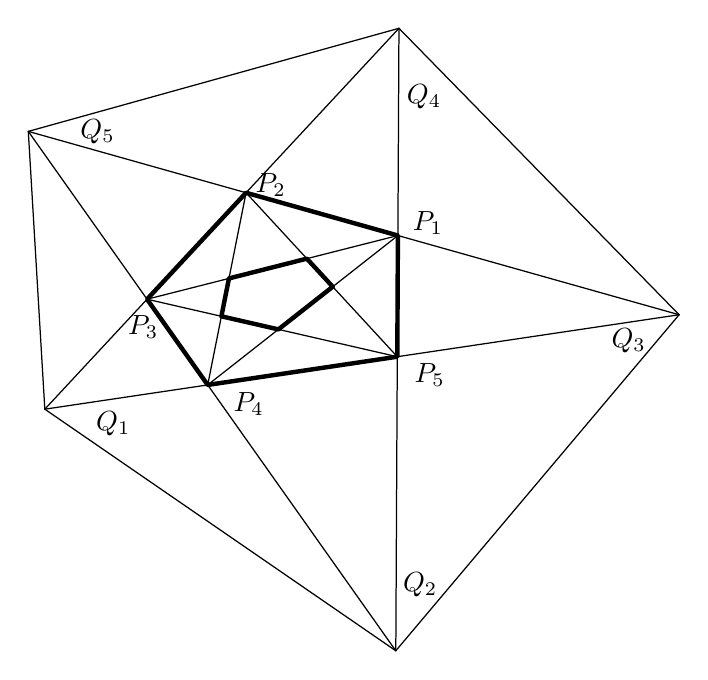
\begin{tikzpicture}[x=.01cm,y=-.01cm,line width=.45pt,line cap=round,line join=round,every node/.style={inner sep=0pt,font=\normalsize}]
\coordinate (Q5) at (392,534);
\coordinate (Q4) at (863,403);
\coordinate (Q3) at (1219,767);
\coordinate (Q2) at (859,1194);
\coordinate (Q1) at (413,887);
\coordinate (P2) at (668.717,611.962);
\coordinate (P1) at (861.668,666.325);
\coordinate (P5) at (860.89,820.317);
\coordinate (P4) at (619.971,856.186);
\coordinate (P3) at (542.909,747.276);
\draw (Q5)--(Q4);
\draw (Q4)--(Q3);
\draw (Q3)--(Q2);
\draw (Q2)--(Q1);
\draw (Q1)--(Q5);
\draw (Q5)--(Q3);
\draw (Q3)--(Q1);
\draw (Q1)--(Q4);
\draw (Q4)--(Q2);
\draw (Q2)--(Q5);
\draw (P2)--(P5);
\draw (P5)--(P3);
\draw (P3)--(P1);
\draw (P1)--(P4);
\draw (P4)--(P2);
\draw[line width=1.6pt] (P2)--(P1)--(P5)--(P4)--(P3)--cycle;
\draw[line width=1.6pt] (646.984,720.845)--(745.96,695.71)--(778.856,731.376)--(709.811,785.614)--(637.377,768.975)--cycle;
\node at (480,534) {$Q_5$};
\node at (895,490) {$Q_4$};
\node at (1155,800) {$Q_3$};
\node at (890,1110) {$Q_2$};
\node at (500,905) {$Q_1$};
\node at (700,602) {$P_2$};
\node at (900,650) {$P_1$};
\node at (902,844) {$P_5$};
\node at (672,880) {$P_4$};
\node at (538,783) {$P_3$};
\end{tikzpicture}
\end{center}

under the collineation

\[
x' = \dfrac{2\,G-1}{2\,G'-1}\,x, \qquad y' = \dfrac{2\,G-1}{2\,G''-1}\,y\tag{5}
\]

maps to itself. See the accompanying figure for illustration. \textsc{Gauss} himself made drawings of this kind in which the pentagonal networks extend much farther. The coefficients on the right of (5) are the »contraction exponents« or »contraction coefficients« occurring in [9] and [10]. It is natural to view the situation in terms of the modern theory of discontinuous substitution groups. The origin $O$ then appears as the inner limit point of the pentagram network and is one of the three limit points of the cyclic collineation group arising from (5).

By the preceding observation, the same situation occurs for every pentagon with reentrant angles. These relations are well known in the more recent literature.

\textsc{Gauss}'s statements can be confirmed as follows. The outer pentagon immediately adjoining $P_1P_2\,..\,P_5$, namely $Q_1Q_2\,..\,Q_5$, is the same as the one obtained by projecting the spherical pentagon with that name. If $Q_k$ has coordinates $x'_k$, $y'_k$, then, since $\HistAngle\,Q_kMP_{k+1} = \dfrac{\pi}{2}$, the five equations hold

\[
x'_k x_{k+1} + y'_k y_{k+1} + 1 = 0.
\]

Comparison with the five equations (4) indicates that formulas (5) are correct for all indices $k$.

\SourceLeaf{124}
Fragment [11] in particular suggests that \textsc{Gauss} recognized the projective character of the developments last discussed. Here \textsc{Gauss} applies the principles of \textsc{Moebius}'s barycentric calculus to the figure of the rectilinear pentagram. \textsc{Gauss}'s formulas are readily understood in terms of this calculus. In keeping with the projective character of the calculus, the starting point is an arbitrary pentagon. According to a letter to \textsc{Schumacher} dated 15 May 1843, \textsc{Gauss} became acquainted only on 14 May of that year with \textsc{Moebius}'s work on barycentric calculus (published in 1827), presumably in connection with the problem of constructing the center of a conic given by five points. For the special pentagon networks to which the formulas in fragments [5] through [10] refer, this task would be identical with the problem of constructing the inner limit point of the individual network. The developments in fragments [7] and [8] date from April 1843, and the development in fragment [11] follows 14 May 1843, probably immediately. We may therefore assume that the investigations recorded in [9] and [10] were carried out in the weeks between the two dates.

\hfill\textsc{Fricke}.

\noindent\hrulefill\par

\end{document}
